\documentclass[crop,tikz]{standalone}
\usetikzlibrary{backgrounds}
\colorlet{blue}{cyan}
\tikzset{
  inverted/.style = {
    color=white,
    background rectangle/.style={fill},
    show background rectangle
  }
}

\tikzset{>=latex}
\usetikzlibrary{shapes}

\begin{document}
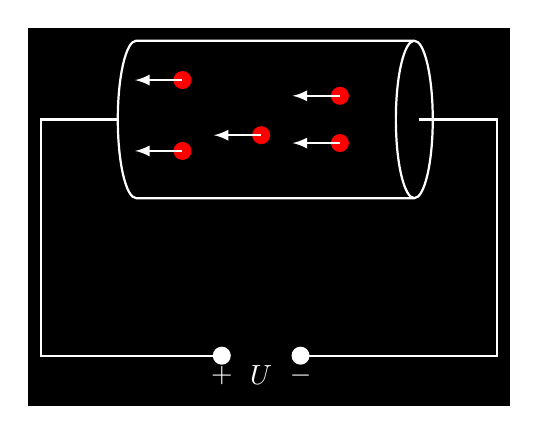
\begin{tikzpicture}[inverted,thick]
  \node (A) at (0,0) [cylinder, aspect=2, shape border rotate=0, draw, minimum height=4cm, minimum width=2cm] {};
  \draw (-1.8,0) -- ++(-1,0) -- ++(0,-3) -- ++(+2.3,0) coordinate (p1);
  \draw (+2,0)   -- ++(+1,0) -- ++(0,-3) -- ++(-2.5,0) coordinate (p2);
  \draw[fill=white] (p1) circle (0.1) node[below] {$+$};
  \draw[fill=white] (p2) circle (0.1) node[below] {$-$};
  \node[below] at (0,-3) {$U$};
  \foreach \x/\y in { -1/-0.4,-1/0.5,0/-0.2,1/0.3,1/-0.3 } {%
    \draw[fill,red] (\x,\y)  circle (0.1) coordinate (t);
    \draw[->] (t) -- ++(-0.6,0);
  }
\end{tikzpicture}
\end{document}
